% LTeX: language=de-DE
\pdfpcnote{
	@Mik \\
	\\
	- Zusaetzlich zum Tree-walking Interpreter haben wir für rush auch noch eine **Virtuelle Maschine** implementiert \\
}
\section{Virtuelle Maschine}

\begin{frame}{Etappen der Übersetzung: Code-Erzeugung}
	\pdfpcnote{
		@Mik \\
		\\
		- Wichtig ist, hierbei handelt es sich um das erste Projekt, welches **Code-Erzeugung**, das heisst **einen Compiler** benoetigt \\
	}
	\begin{figure}[h]
		\begin{adjustbox}{max totalsize={\textwidth}{!},center}
			\begin{tikzpicture}[node distance=3mm and 1cm, inner sep=3mm]
				\node (syntactic_analysis_text) [inner sep=0] {Syntaxanalyse};
				\node (lexical_analysis) [rec, below=of syntactic_analysis_text] {Lexikalische Analyse};
				\node (syntactic_analysis) [rec, fit={(syntactic_analysis_text) (lexical_analysis)}] {};
				\node (semantic_analysis) [rec, right=of syntactic_analysis] {Semantische Analyse};
				\draw [arrow] (syntactic_analysis) -- (semantic_analysis);
				\node (codegen) [rec, fill=mLightBrown!35, right=of semantic_analysis] {Code-Erzeugung};
				\draw [arrow] (semantic_analysis) -- (codegen);
			\end{tikzpicture}
		\end{adjustbox}
	\end{figure}
\end{frame}

\begin{frame}{Virtuelle Maschine}
	\pdfpcnote{
		@Mik \\
		\\
		- Aber ist eine Virtuelle Maschine nicht ein Programm, was einen echten Computer simuliert? \\
            - Das heisst, es werden auch Geraete wie \\
            - das Display \\
            - die Lautsprecher \\
            - und die Festplatte \\
            - simuliert. \\
		\\
		--- \\
		\\
		- In diesem Kontext ist eine VM **eine Software, die wie die CPU eines Rechners funktioniert** \\

	}
	\begin{itemize}
		\item<1-> Häufig: Eine \emph{Virtuelle Maschine} (VM) simuliert echte Computer
			\begin{itemize}
				\item Display
				\item Lautsprecher
				\item Festplatte
				\item \dots
			\end{itemize}
		\item<2-> Hier: Software, die wie die CPU eines Rechners funktioniert
	\end{itemize}
\end{frame}

\begin{frame}{Virtuelle Maschine}
    \pdfpcnote{
        @Mik \\
        \\
        - Hier ist der Ablauf aehnlich wie der des Compilers \\
        - Zuerst wandelt der Compiler das Programm in ein anderes Format um, welches die VM versteht \\
        - Diese fuehrt dann anschliessend das Ausgabeprogramm aus \\
        - Somit funktioniert die VM wie eine CPU mit einer eigenen Architektur \\
        \\
        --- \\
        \\
        - Dies wirkt von Aussen allerdings wie ein Schritt, weshalb wir die VM als Interpreter einordnen \\
        - Sprachen, die aehnlich funktionieren, sind zum Beispiel **Java** \\
    }

	\hspace{.3cm}
	\begin{minipage}{.2\textwidth}
		\begin{center}
			\Lirsting[float=H, fancyvrb={frame=none, fontsize=\footnotesize}]{deps/paper/listings/simple.rush}
		\end{center}
	\end{minipage}%
	\hspace{-.3cm}
	\Larrow{
		\begin{minipage}{1.3cm}
			Compiler
		\end{minipage}
		\begin{minipage}{5mm}
			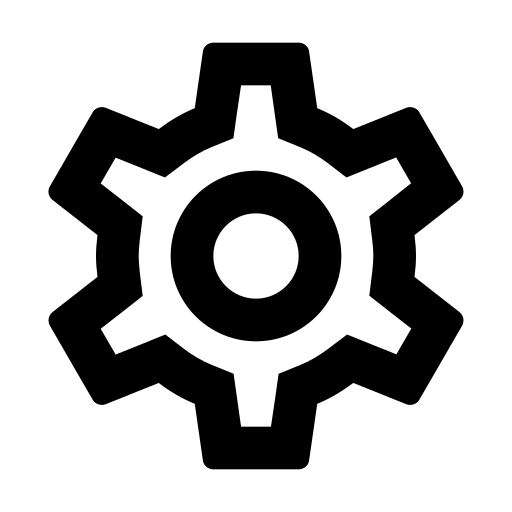
\includegraphics[width=3.5mm]{assets/google_icon_settings.png}
		\end{minipage}
	}
    \hspace{.8cm}
	\begin{minipage}{.24\textwidth}
		\Lirsting[float=H, fancyvrb={frame=none, fontsize=\footnotesize}, ranges={4-20}]{listings/simple_vm.s}
	\end{minipage}
	\Larrow{
		\begin{minipage}{.4cm}
			VM
		\end{minipage}
		\begin{minipage}{5mm}
			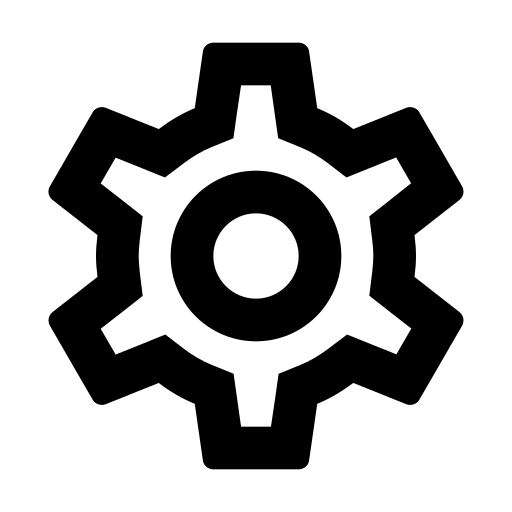
\includegraphics[width=3.5mm]{assets/google_icon_settings.png}
		\end{minipage}
	}
    \hspace{.1cm}
	\begin{minipage}{.13\textwidth}
		\centering
		{\large Exit code: 5}
	\end{minipage}
	\hfill

	\begin{itemize}
		\item Java, usw.
		\item Umwandlung in ein anderes Format
		\item[\Rightarrow] Anschliessende Ausführung des Programmes
	\end{itemize}
\end{frame}

\begin{frame}{Die rush VM}
	\pdfpcnote{
		@Mik \\
		\\
        - Diese Konzepte wurden nun auch auf die rush VM uebertragen \\
        \\
        --- \\
        \\
        1. Hier werden auch vorher uebersetzte Programme ausgefuehrt \\
		2. Die VM besitzt **eine selbst entwickelte Architektur**, die das Ziel des Compilers darstellt \\
		    - Diese Architektur besitzt ein **stackbasiertes Design** und einen **hohen Abstaktionsgrad** \\
	}
	\begin{itemize}
		\item<1-> Führt ein zuvor übersetztes Programm aus
		\item<2-> Besitzt eine selbst entwickelte Architektur
		      \begin{itemize}
			      \item Stackbasiertes Design
			      \item Hoher Abstaktionsgrad
		      \end{itemize}
	\end{itemize}
\end{frame}

\begin{frame}{Felder der VM}
    \pdfpcnote{
        @Mik \\
        \\
        - Im Vergleich zum Tree-walking Interpreter hat die VM 4 Felder \\
        \\
        --- \\
        \\
        1. Einen **stack** fuer temporaere Werte \\
        2. Die Felder **mem** und **mem-ptr** zur Speicherung von Variablen \\
        3. Einen **call-stack**, also einen Aufrufstapel, der mehrere **Befehlszaehler** und **Funktionszaehler** verwaltet \\
    }
	\begin{description}
		\item<1->[stack] Für temporäre Werte
		\item<2->[mem] Für Variablen
		\item<2->[mem\_ptr] Für Speicherverwaltung
		\item<3->[call\_stack] Aufrufstapel (\emph{Befehlsähler} und \emph{Funktionszähler})
	\end{description}
\end{frame}

\begin{frame}{Struktur der Programme der rush VM}
    \pdfpcnote{
        @Mik \\
        \\
        - Ein Teil der Architektur der VM ist die Struktur ihrer Programme... \\
        \\
        --- \\
        \\
        - Die Programme sind in Funktionen aufgeteilt \\
            - Diese haben keinen Namen aber eine numerische Identifizierung \\
            - Jede Funktion enthaehlt mehrere Anweisungen \\
        -  Jede Anweisung ist wie folgt aufgebaut: \\
            - Als Beispiel betrachten wir die Anweisung **call 2** \\
            - Der Befehlscode, also **call** \\
            - Und ein optionaler Operand, hier die **2** \\
        - Nach dem neusten Stand der Entwicklung besitzt die VM gerade einmal ca. 30 verschiedene Befehlscodes \\
    }
	\begin{itemize}
		\item<1-> Unterteilung in Funktionen
			\begin{itemize}
				\item Ohne Namen
				\item numerische Identifizierung
				\item Enthält mehrere Anweisungen
			\end{itemize}
		\item<2-> Struktur der Anweisungen: \enquote{\LirstInline{asm}{call 2}}
			\begin{itemize}
				\item<2-> Befehlscode (\texttt{call})
				\item<2-> Optionaler Operand (\texttt{2})
			\end{itemize}
		\item<3-> ca. 30 verschiedene Befehlscodes
	\end{itemize}
\end{frame}

\begin{frame}{Demonstration: Ein-/Ausgabe}
	\begin{minipage}{0.5\textwidth}
		\Lirsting[float=H, fancyvrb={frame=none, fontsize=\small}]{deps/paper/listings/fib.rush}
		\centering
		\Larrow{Ausgabe}
	\end{minipage}
	\hfill
	\begin{minipage}{0.35\textwidth}
		\Lirsting[float=H, fancyvrb={frame=none, fontsize=\footnotesize}, ranges={1-20,26-32}]{listings/vm_fib.s}
	\end{minipage}
\end{frame}

\begin{frame}{Demonstration: Laufzeitverhalten}
	\begin{figure}[H]
		\href{run:assets/01_rush_presentation_vm.mkv}{
			\movie{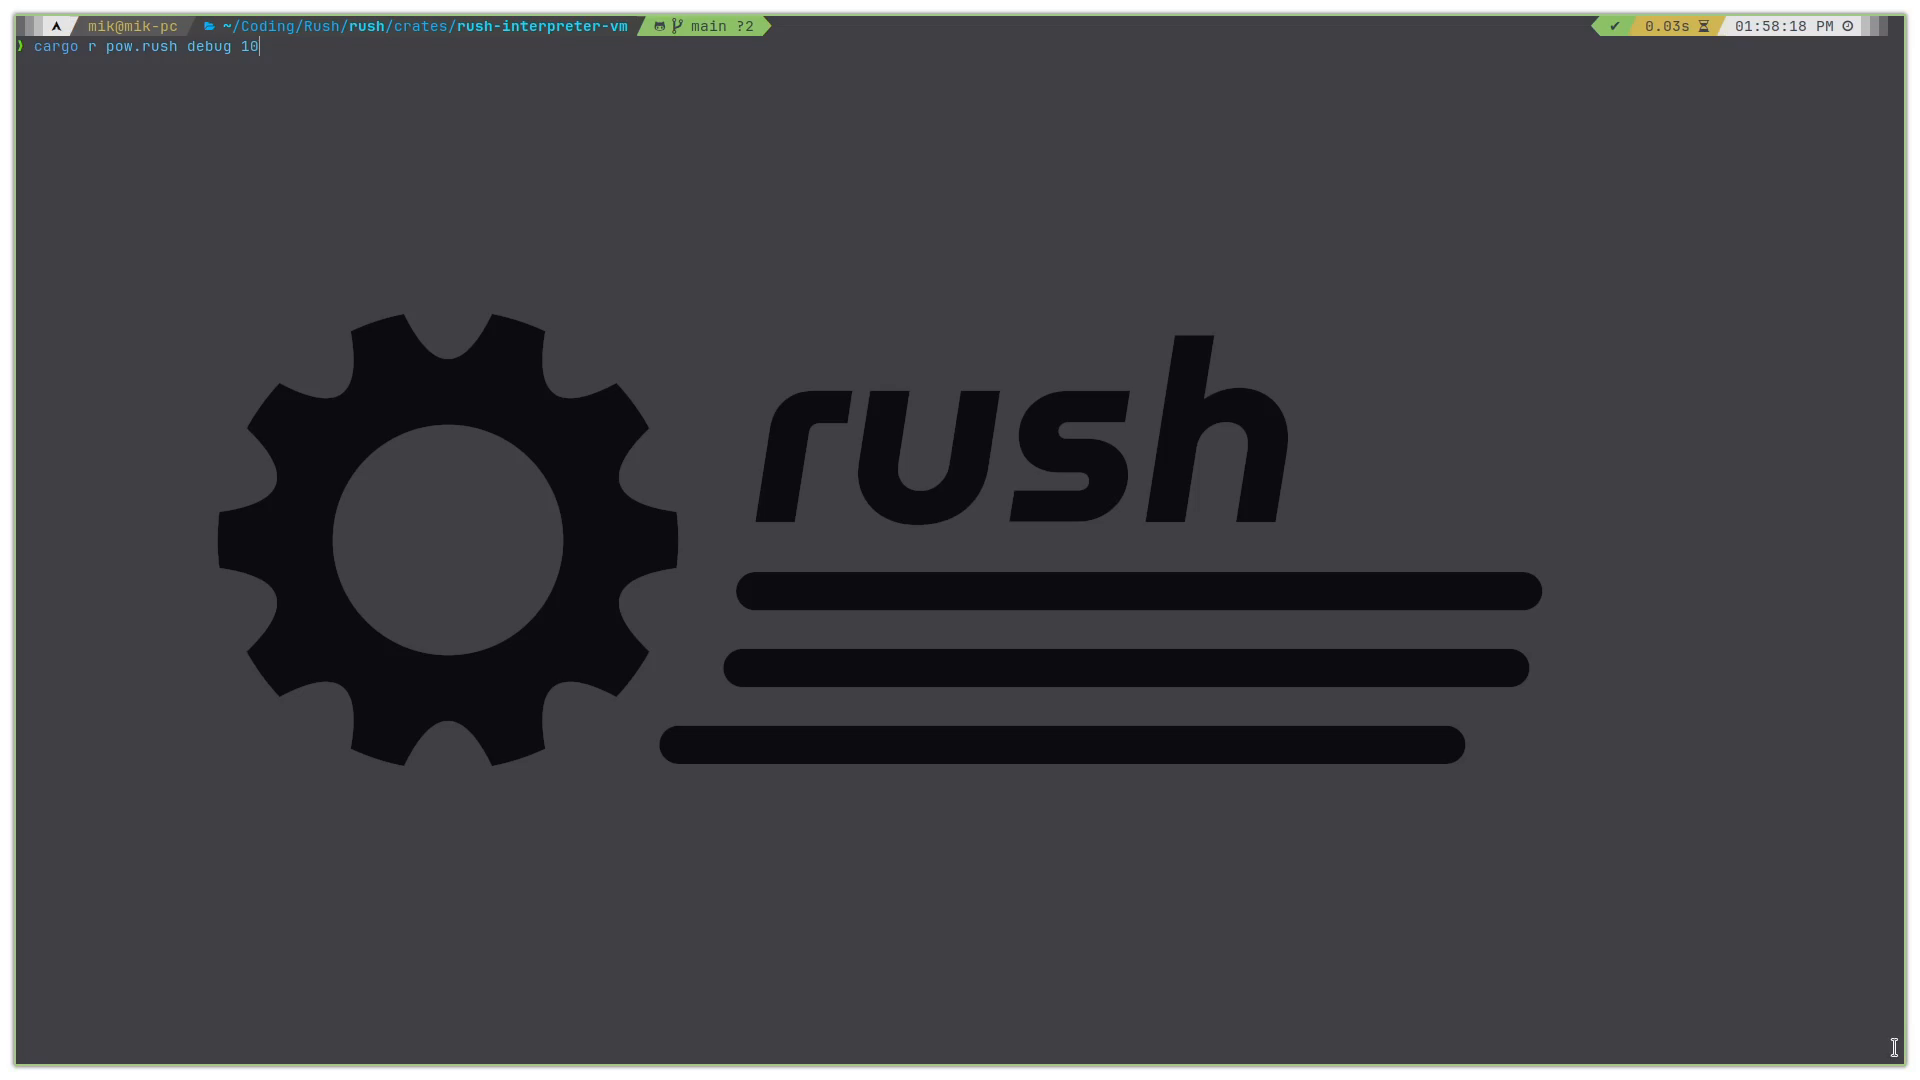
\includegraphics[width=.95\textwidth]{assets/01_rush_presentation_vm.png}}{assets/01_rush_presentation_vm.mkv}
		}
	\end{figure}
\end{frame}

\begin{frame}{VM: Fazit}
	\begin{itemize}
		\item<1-> Ca. 2.7 mal schneller als der Tree-walking Interpreter
		\item<2-> Einfache Implementierung des Compilers
			\begin{itemize}
				\item<3-> Stack-basierte Architektur
				\item<4-> Gleichzeitige Entwicklung von VM und Compiler (\cemph{Feedbackschleife})
				\item<5-> Hoher Abstraktionsgrad
			\end{itemize}
	\end{itemize}
\end{frame}
